
\chapter{Fundamentação} \label{ch:fundamentation}

Este Capítulo apresenta a fundamentação necessária para o entendimento do trabalho. 
Ele é separado em duas Seções, na primeira, são apresentadas as ferramentas de análise de
desempenho de aplicações paralelas e, na segunda, são contextualizadas ferramentas que
serão utilizadas no trabalho.

\section{Análise de desempenho de aplicações paralelas}

Nesta Seção, serão apresentados os trabalhos relacionados. Eles foram agrupados em duas
categorias, a primeira delas, \emph{
Ferramentas de visualização Clássicas}, consiste em ferramentas que oferecem visualização de \emph{traces} de aplicações desenvolvidas no modelo BSP. A segunda, denominada \emph{Ferramentas de visualização orientadas a tarefas} oferecem visualização de traces de aplicações desenvolvidas no modelo orientado a tarefas. Nas próximas subseções, serão detalhados os trabalhos de cada um desses grupos.

\subsection*{Ferramentas de visualização Clássicas}

Essas ferramentas possuem o objetivo de prover visualizações de traces para aplicações de HPC tradicionais. Estas eram desenvolvidas
seguindo o modelo que consiste em uma série de \emph{supersteps} (computações, comunicações, sincronizações), executadas com a premissa de ter-se um ambiente homogêneo, denominado \emph{Bulk-Synchronous Parallel}. Como esta abordagem  dominou o cenário HPC durante muito tempo, suas necessidades
balizaram o desenvolvimento da maior parte das ferramentas de análise de desempenho.

\subsubsection*{ViTE}
ViTE \cite{ref:vite} é uma ferramenta de visualização de \emph{traces} open-source. Para o processamento de grandes entradas ele conta com aceleração de Hardware e OpenGL. Suas entradas são arquivos na linguagem Pajé \cite{ref:paje}.

Essa ferramenta exibe os recursos de forma hierárquica, onde oferece a visualização das tarefas (eixo vertical) em função de tempo (eixo horizontal), similar a um Gantt. Na análise de aplicações distribuídas, também é possível incluir indicadores de transferências de dados.

\subsubsection*{Paraver}
Paraver \cite{ref:paraver} também objetiva a visualização e análise de \emph{traces} de execução. Ela conta com uma agregação de dados, definida pelo
usuário via arquivo de configuração, para conseguir exibir entradas volumosas. Suas entradas são geradas por vários modelos de programação, pela ferramenta Extrae.

\subsubsection*{Vampir}
Vampir \cite{ref:vampir} é uma ferramenta proprietária de código fechado para fins de análise de \emph{traces}. Ela traz uma abordagem de cliente-servidor, onde o servidor pode ser executado no hardware de experimentação e o cliente é o computador do usuário.

Suas entradas são arquivos OTF2 (Open Trace Format, version 2) \cite{ref:otf2}. Ele fornece múltiplas visualizações como gráficos de espaço-tempo e estatísticas de execução.

\subsubsection*{Ravel}
O objetivo da ferramenta Ravel \cite{ref:ravel} também é a visualização de \emph{traces}. Suas entradas são em formato OTF \emph{Open Trace Format} e sua diferença em relação aos demais é que ele mostra as linhas de tempo lógicas, fornecendo uma estruturação para melhor entendimento de operações.

\subsubsection*{FrameSoc e Ocelotl}

FrameSoc \cite{ref:framesoc} é uma ferramenta de análise de performance, capaz de lidar com grandes volumes de dados. Como entrada, ela suporta diversos
formatos como Pajé, CTF, Paraver e OTF2. Além dos dados de \emph{trace}, é possível armazenar informações como metadados e anotações. A ferramenta converte tudo para um modelo de dados genérico e armazena em uma base de dados relacional.

Para visualizar grandes volumes de dados, a ferramenta baseia-se no Ocelotl \cite{ref:ocelotl}. Esse módulo possui um arquivo de configuração parametrizável pelo usuário, que gerencia uma agregação espaçotemporal dados.

\subsection*{Ferramentas de visualização orientadas a tarefas}

Como os recursos e o custo de execução de tarefas não são constantes no modelo \emph{task-based}, é necessário representações diferentes para
possibilitar uma análise de performance nesses ambientes. O desenvolvimento do \emph{framework} StarVZ \cite{ref:starvz} foi motivado pela carência
de ferramentas maduras para a visualização de \emph{traces} com o objetivo de identificação de melhorias de performance. Antes de seu desenvolvimento existiam algumas ferramentas, todavia, elas não forneciam dados suficientes para identificar otimizações de forma eficiente.

\subsubsection*{DAGViz}

DAGViz \cite{ref:dagviz} é composto por dois passos: 

\begin{enumerate}
    \item extração do DAG dos arquivos de uma execução paralela;
    \item visualização hierárquica do DAG.
\end{enumerate}

Essa ferramenta traz uma visualização diferente do modelo BSP, exibindo as tarefas como um grafo hierárquico. Nele, o analista pode colapsar e expandir os grupos de tarefas. Dados de tempo de execução não são tratados pela ferramenta.

\subsubsection*{Traces de execução com dependências de tarefas}

A ferramenta desenvolvida por \citet{ref:visuexecdep} traz um gráfico no estilo espaço-tempo (Gantt). Há algumas outras funcionalidades como a identificação de dependências de tarefas (apenas o primeiro nível) a medida que o usuário passa o mouse sobre as caixas que representam as tarefas.

Como entradas, são utilizados a representação do DAG e os \emph{traces} de execução. Essa ferramenta é desenvolvida para o especificamente para o \emph{runtime} PaRSEC.

\subsubsection*{Temanejo}

Temanejo \cite{ref:temanejo} é um \emph{debugger} para o modelo de programação baseado em tarefas, onde o analista visualiza um DAG. Ele suporta grande parte dos 
\emph{runtimes} de execução de aplicações baseadas em tarefas, como OmpSs, StarPU e PaRSEC. Suas funcionalidades são focadas em depuração, permitindo que o usuário possa identificar e consertar parâmetros e dependências de tarefas.

\subsubsection*{Delay Spotter}

Delay Spotter \cite{ref:delayspotter} é uma ferramenta, construída sobre o DAGViz, que possibilita a identificação de atrasos em \emph{runtimes}.
Ela divide os estados dos \emph{workers} em três categorias, permitindo a identificação de delays decorrentes de problemas de escalonamento.
Como em ambientes heterogêneos com tarefas variadas, a presença de \emph{delays} faz parte da execução das aplicações, essa ferramenta é pouco efetiva.

\subsubsection*{TaskInsight}

TaskInsight \cite{ref:taskinsight} é uma ferramenta que objetiva identificar o comportamento de memória e seu impacto na execução de tarefas. 
Apesar de prover algumas estatísticas e possibilitar algumas identificações de anomalias, apenas essa análise não é o suficiente para
identificar a maioria dos pontos de otimização de aplicações \emph{task-based}.

\subsubsection*{StarVZ}

\emph{Framework} que é objeto deste trabalho, o StarVZ \cite{ref:starvz} possui a visualização de dados mais avançada dentre as ferramentas citadas.
Construído com uma abordagem de \emph{script}, ela possui um grande poder de customização e, por isso, é difícil enumerar o que a ferramenta fornece.
No trabalho de \citet{ref:starvz}, podemos visualizar diversos gráficos gerados de uma execução de aplicação:

\begin{itemize}
    \item gráfico com comportamento de tarefas;
    \item gráfico com a quantidade de tarefas submetidas;
    \item o comportamento do \emph{runtime}, com os estados dos \emph{workers} StarPU;
    \item a quantidade de tarefas prontas;
    \item taxa de GFlops do ambiente;
    \item tráfego de dados entre a memória das GPUs;
    \item transferências de rede MPI;
    \item número de operações MPI concorrentes.
\end{itemize}

Ele é composto por dois passos, como podemos observar na Figura \ref{fig:starvz-steps}. O primeiro, executado em um servidor e cujo objetivo é fazer um pré-processamento dos dados. O segundo é realizado diretamente na máquina do analista, trata-se apenas de manipulações para visualização.

\begin{figure}[H]
 \centerline{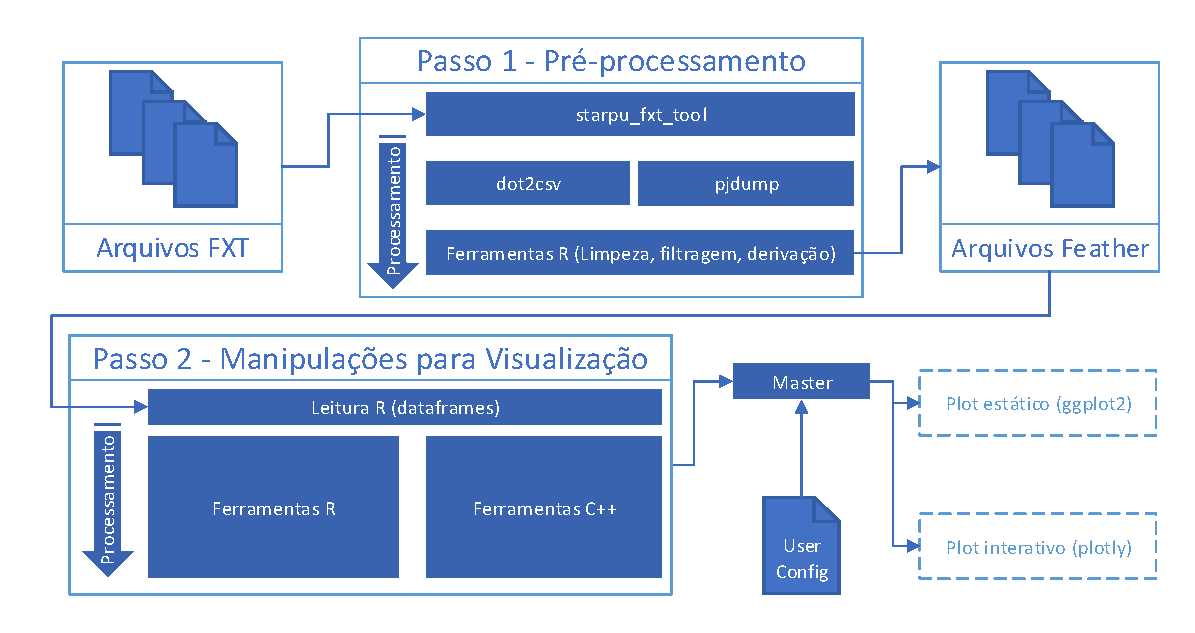
\includegraphics[width=1\textwidth]{./images/all-proc.pdf}}
 \caption{Passos de processamento do StarVZ}
 \label{fig:starvz-steps}
\end{figure}


















\section{Conceitos Básicos} \label{sect:basic-concepts}

O StarVZ \cite{ref:starvz} é um \emph{workflow} de análise de performance cujo 
objetivo é auxiliar na avaliação e na verificação de hipóteses sobre a execução de 
aplicações \emph{task-based} em ambientes heterogêneos, executados sobre o
\emph{runtime} StarPU \cite{ref:starpu}. Ele é composto de duas fases, cada uma 
delas composta de uma combinação de diversas ferramentas, resultando em um \emph{framework}
rápido, consistente, flexível e versátil.

Na primeira fase, que pode ser visualizada na Figura \ref{fig:starvz-workflow1}, os 
\emph{Execution Traces} do StarPU, que são arquivos em um formato binário, são transformados
e exportados através da ferramenta \texttt{starpu\_fxt\_tool} para dois arquivos: DAG no formato DOT 
e Trace no formato PAJE. Essa etapa gera eventos com informação de data e hora, que 
descrevem o comportamento da aplicação para todos os recursos envolvidos. Também são gerados 
dados sobre o \emph{runtime} do StarPU, como número de tarefas submetidas,
número de tarefas prontas, arquitetura da plataforma, etc.

\begin{figure}[ht]
 \centerline{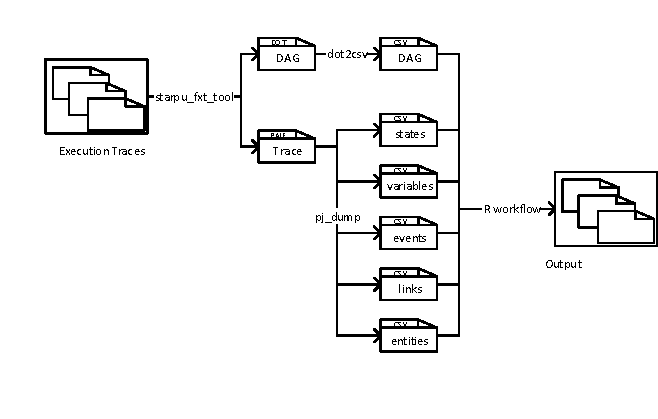
\includegraphics[width=1\textwidth]{./img/step1-final.pdf}}
 \caption{\emph{Workflow} de pré-processamento do StarVZ.}
 \label{fig:starvz-workflow1}
\end{figure}

Em seguida, é realizada uma verificação de integridade estrutural e temporal dos
arquivos \emph{trace}. Ela é executada via \texttt{pj\_dump}, gerando cinco arquivos: o arquivo states 
possui informações sobre as tarefas executadas e seu comportamento no \emph{runtime}; variables
consiste em métricas de performance da plataforma e \emph{runtime}; events possui informações sobre a 
utilização de recursos; links contém dados sobre comunicação MPI; e as informações de plataforma 
são registradas no arquivo entities. O DAG também passa por uma conversão e por fim, todos os 
arquivos são gravados no formato \emph{Comma-Separated Value} (CSV).

Finalmente, os dados escritos em CSV são lidos, filtrados, agregados e combinados em 
uma ferramenta implementada na linguagem R, utilizando-se bibliotecas oriundas do pacote 
\texttt{tidyverse} para a manipulação de dados. As saídas são escritas no formato \emph{FEATHER}
\cite{ref:feather}.

A segunda fase do \emph{workflow} inicia pela leitura das saídas da anterior. Cada arquivo
torna-se um \emph{data frame}, e os dados da execução inteira são unificados em uma estrutura.
É possível ter múltiplos \emph{traces} de aplicações sendo analisados em paralelo
para comparação, basta multiplicar a leitura com entradas diferentes e 
elas podem posteriormente ser combinadas em uma única visualização. A criação dos gráficos ainda 
possui processamento de dados, o que traz certa flexibilidade para as visualizações. Como última etapa dessa fase, o usuário 
parametriza o sistema com um arquivo de configuração no formato YAML, para que a montagem da visualização seja customizada. Finalmente, o usuário pode analisar os gráficos gerados pela ferramenta.

Nos experimentos realizados em \citet{ref:starvz}, em uma máquina equipada com um Intel(R) Xeon(R) 
CPU E3-1225 v3 @3.20GHz e 32GB de memória principal e com uma entrada de aproximadamente 18GB, a 
primeira fase do \emph{workflow} levou cerca de 32 minutos para executar: a execução da \texttt{starpu\_fxt\_tool}
levou em torno de 10 minutos, o \texttt{pj\_dump} levou cerca de 9 minutos e a ferramenta R levou cerca de 13
minutos. Já a segunda fase do \emph{workflow}, para executar a leitura dos arquivos \emph{FEATHER} e gerar
a visualização levou em torno de 2 minutos.

\section{Trabalhos Relacionados}\label{sect:related-work}

O trabalho de \citet{ref:drakestarvz} foi o primeiro a tentar otimizar o fluxo do StarVZ. 
Sua principal motivação foi a melhoria de performance da etapa de manipulação de dados, a mais
custosa de acordo com os experimentos observados, com o objetivo de permitir o processamento de 
entradas maiores em um tempo aceitável.

Nele utilizou-se \texttt{Drake} \cite{ref:drake}, uma biblioteca para a linguagem de programação R, cujo foco é executar apenas as 
partes necessárias de um \emph{workflow} de análise de dados, evitando os passos desnecessários que não mudarão
suas saídas. Isso é realizado modelando as computações como um \emph{directed acyclic graph} (DAG) de tarefas e 
armazenando em cache os resultados daquelas já executadas. Além disso, \texttt{Drake} também possui suporte a paralelismo
(\emph{Implicit parallelism}) para a execução de tarefas independentes.

Para modelar o StarVZ dessa forma, foram necessárias mudanças cujo objetivo era explicitar 
dependências e postergar junções de \emph{data frames}. Depois da identificação dos fluxos independentes    
no \emph{workflow}, foi utilizado \texttt{Drake} para criar um plano de execução, que consiste na declaração
das tarefas onde cada uma é representada por uma função R. Na criação do plano, a biblioteca analisa cada
uma das tarefas, suas entradas e saídas, para determinar dependências e gerar o DAG. O resultado da modelagem do
StarVZ nessa abordagem pode ser visualizado na Figura \ref{fig:starvz-dag}.

\begin{figure}[ht]
 \centerline{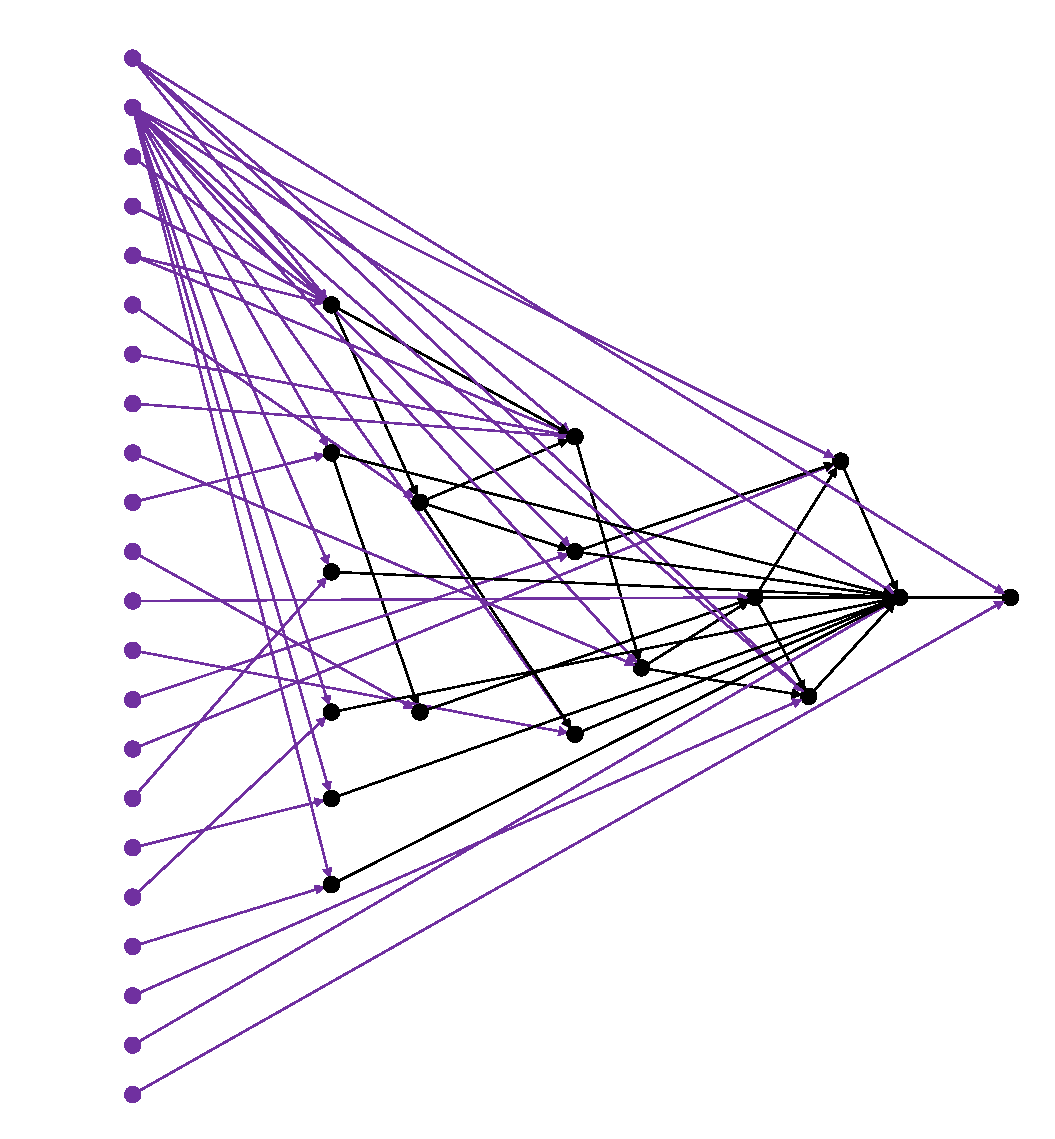
\includegraphics[width=0.8\textwidth]{./img/drake-dag-final-origin.pdf}}
 \caption{DAG de execução do StarVZ.}
 \legend{Fonte: Inspirada na Figura de contida no trabalho de \citet{ref:drakestarvz}}
 \label{fig:starvz-dag}
\end{figure}

Com esta modelagem, não foram observadas melhorias de performance no StarVZ. De acordo com \citet{ref:drakestarvz},
a cache de resultados intermediários da biblioteca acaba tendo que armazenar muitos dados em disco devido
ao tamanho dos \emph{data frames} gerados pelas entradas, prejudicando o tempo total de processamento.
Em relação ao suporte a paralelismo, ele é limitado pela falta de suporte nativo a \emph{multithread} da linguagem R.
Por isso, \texttt{Drake} oferece essa funcionalidade instanciando múltiplas sessões R, que são processos separados. A comunicação
entre esses processos é realizada pelo mesmo sistema de cache citado anteriormente, consequentemente, resultando nos mesmos
problemas.

Outra abordagem que poderia ser adotada para melhorar o desempenho do StarVZ seria distribuir os fluxos independentes
do \emph{workflow} pois elas podem trazer um ganho de desempenho em um ambiente viável.
Ao simplesmente paralelizar, é possível que os mesmo problemas com o tamanho dos \emph{data frames} sejam enfrentados, exigindo
máquinas com muita memória para obter-se os resultados desejados. 

A primeira opção seria distribuir os fluxos independentes utilizando o pacote \texttt{Snow}, que significa 
\emph{Simple Network of Workstations} \cite{ref:snow}. Este é desenvolvido para linguagem R e permite a utilização
de \emph{Explicit parallelism}, oferecendo integração com três interfaces de baixo nível: PVM (\emph{Parallel Virtual Machine}), através do pacote rpvm; MPI, através do pacote Rmpi \cite{ref:rmpi}; e uma integração com sockets, no caso de não ter nenhuma das outras 
opções disponíveis no ambiente. A utilização de \texttt{Snow} pode ser feita através da biblioteca \texttt{Snowfall} \cite{ref:snowfall},
que é um \emph{usability wrapper}, facilitando ainda mais a utilização.

A segunda alternativa seria a utilização da biblioteca \texttt{future} \cite{ref:future}. Esta provê uma forma simples e uniforme 
de avaliar expressões de forma assíncrona, utilizando recursos diversos. Ela funciona utilizando o conceito de abstração 
\emph{future}, que básicamente define um valor que poderá estar disponível no futuro. Tal valor pode ter seu estado como 
resolvido ou não resolvido, estado em que se ele for utilizado bloqueará o processo até sua resolução. Os \emph{futures} 
podem ser resolvidos de diversas formas: sequential, onde são resolvidos sequencialmente no processo R corrente; multiprocess,
que resolve utilizando \emph{multicore}; cluster, que é o mais interessante para adoção pois resolve com sessões R na máquina 
local e/ou em máquinas remotas; e etc.